
\clearpage{}
\section{Update without imperative variables}
\label{System:Update}
In a typical imperative language the syntax to bind a variable is the same as that used to update it. This conflates the two issues. Consider the semantics of the following program fragment:

\code{
	$x = 5$
}

Readers with a more functional background would likely read this as ``$x$ has value 5''. Readers with a more imperative background could equally reply ``$x$ is being updated to value 5.'' With the difference between boxed and unboxed integers in mind, the fragment could also mean ``$x$ is a pointer to an object, and it is the pointer which is being updated'' or perhaps ``$x$ points to an object, and it is the \emph{object} which is being updated''. These three readings for update are shown in the following diagram, where the value is being updated from 3 to 5.

\begin{center}
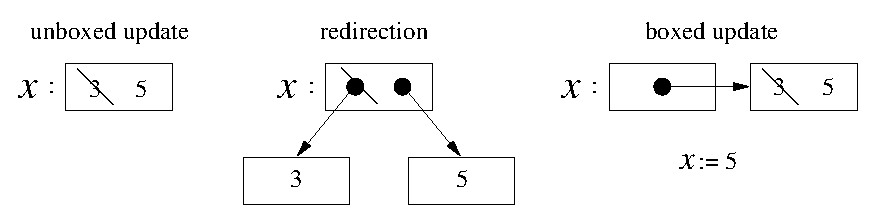
\includegraphics[scale=0.8]{2-System/fig/updateOperators}
\end{center}

In the first two cases it is the local value of $x$ that is being changed. In these cases we call $x$ an \emph{imperative variable}, and we do not support this form of update in our language. However, in the last case only the object pointed to by $x$ changes. We support this option and write $x := 5$ to distinguish it from the syntax for \emph{binding} which is simply $x = 5$.

Why do it this way? Firstly, we intend to support update by the inclusion of functions such as:

\code{
	$\iupdateInt$ 	& $::$ & $\iInt \to \iInt \to ()$ \\
	$\iupdateChar$ 	& $::$ & $\iChar \to \iChar \to ()$
}

The first parameter of these functions is the object to be updated, and the second is the source of the new value. We use $(:=)$ as an overloaded update operator, so $x := 5$ can be rewritten as $\iupdateInt \ x \ 5$.

In light of this, we restrict update to objects for two main reasons. The first is that in our implementation we use local unboxing~\cite{leroy:unboxing} to support efficient numeric computation, and we desire intermediate results to be held in the register set wherever possible. If we permit local values to be updated, then we would also want to pass them by reference, so that called functions could update them via this reference. 

\clearpage{}
Consider then an unboxed version of $\iupdateInt$, and some C code that uses it:

\begin{lstlisting}
    void trouble(void) 
    {
        int x, y;

        ...
        x = 3;
        y = 5;
        updateIntUnboxed (&x, y);
        ...
    }
\end{lstlisting}

This code is valid, though deeply troubling to a C compiler. As $x$ is passed by reference, its value \emph{must} be held on the stack instead of in the register set, otherwise we couldn't construct a pointer to it. More seriously, in regards to separate compilation, a C compiler would be unable to guarantee that this pointer becomes unreachable before \texttt{trouble} returns, losing the stack frame and the storage for \texttt{x}. As in \cite{henderson:accurate} we have observed GCC to disable a number of low-level optimisations when compiling code which uses pointers to automatic variables. We could perhaps implement local update as a primitive of the language, but we avoid this option due to the extra complexity and conceptual mismatch relative to object update.

Another reason for not supporting imperative variables, and perhaps a more convincing one for readers who don't spend all their time writing compilers, is that it simplifies the type system. If we only support update of the objects \emph{pointed to} by our variables then we only need to reason about the mutability of these objects, and not of the variables as well. This can be contrasted with \cite{odersky:less-destructive} and \cite{shapiro:origins-of-bitc} which reason about both.

